\section{Results, Analysis, and Discussion}
\label{appendix:results}

This section presents quantitative results for the experiments described in Appendix~\ref{appendix:protocol}. We emphasize statistical significance, distribution analysis, and practical implications for real-world deployment.



\subsection{Experiment 1: Baseline Performance Results}

Hardware performance was evaluated over 50 trials per controller at 20~Hz
using stratified initial conditions (Section~\ref{sec:ic_design}).
Figure~\ref{fig:hw_ranking} ranks all controllers by success rate;
Figure~\ref{fig:hw_pareto} shows the failure-vs-settling trade-off;
and Figure~\ref{fig:hw_difficulty} decomposes SR by stratum, while
Figure~\ref{fig:settling_by_stratum} does the same for median settling time,
where the pattern is strongly controller-dependent: MPPI stays tight across
strata (1.2--2.7\,s), the wall-override classical controllers mostly slow
toward the boundary (MPC+WO excepted), and the simulation-trained RL agents
swing widely from one stratum to the next, though with only five trials in
each at-wall stratum much of that swing is sampling noise.

\paragraph{Evaluation protocol.}
Every controller in the benchmark received the full 50-trial stratified
evaluation: the five model-free RL algorithms (PPO with BZ+DR; TD3, TQC,
SAC, TRPO with DR), the model-based controllers (MPPI, PPO~(WM)), offline
RL (IQL), and all classical controllers.


\begin{figure}[b]
  \centering
  
\includegraphics[width=0.95\columnwidth]{figures/hw_sr_vs_settling.eps}
  \caption{Hardware failure rate vs.\ median settling time
    (successful trials); both axes increase toward worse outcomes, so
    the ideal controller occupies the bottom-left corner. MPPI ties for the
    best success rate (100\%, with PPO~(WM)) and has the fastest median
    settling (1.67~s); PPO~(BZ+DR) offers 96\% SR with 3.15~s median settling.}
  \label{fig:hw_pareto}
\end{figure}

\begin{figure}[b]
  \centering
  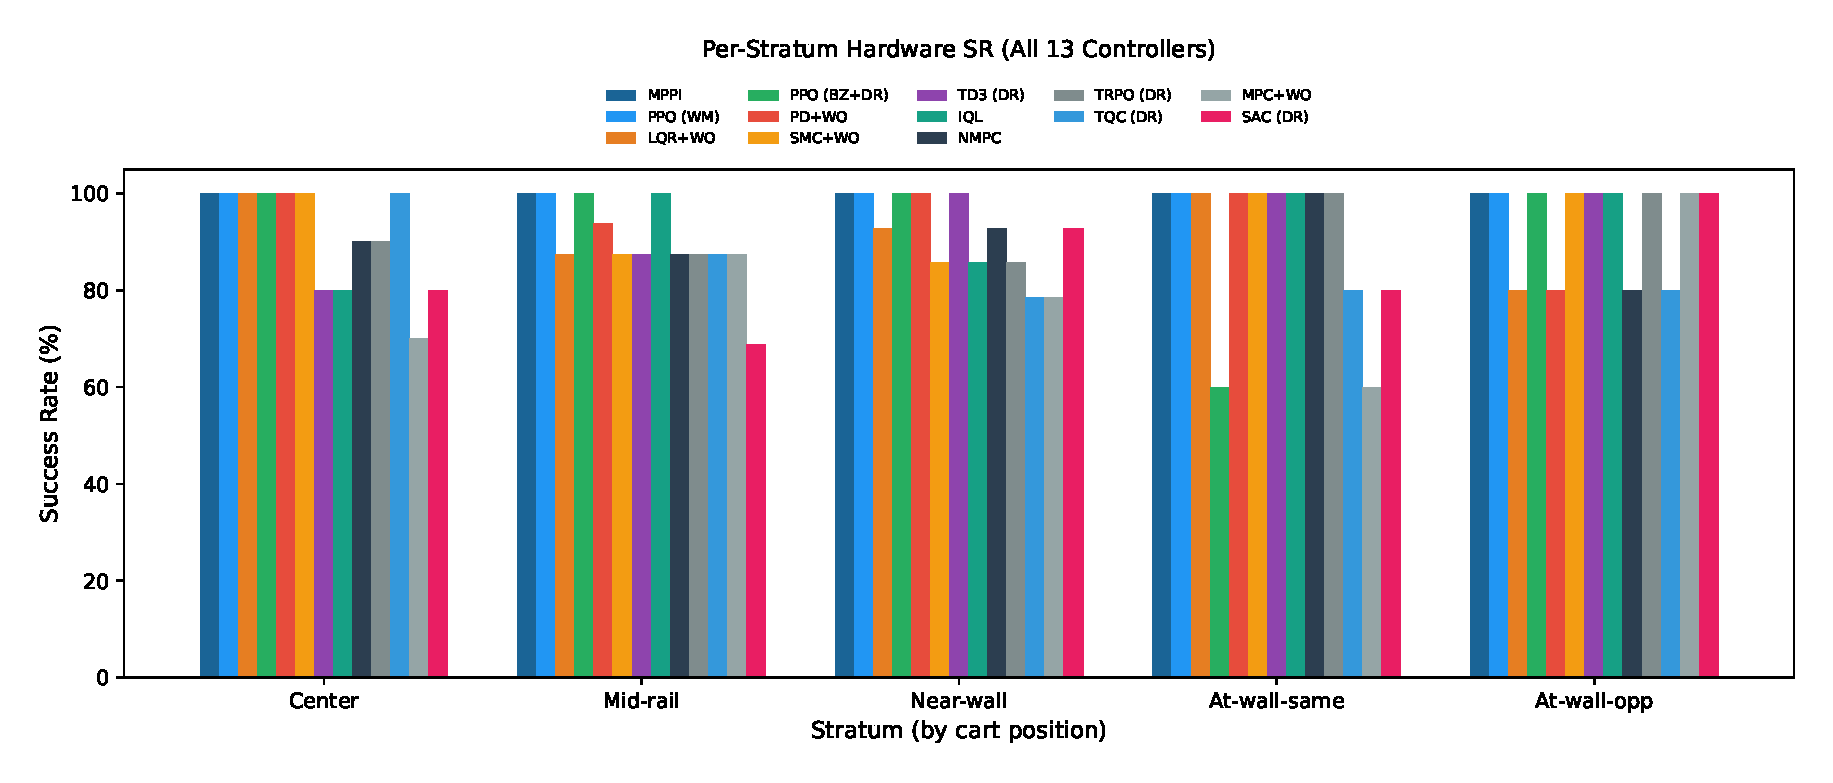
\includegraphics[width=0.95\columnwidth]{figures/settling_by_stratum.eps}
  \caption{Per-stratum hardware SR for all 13 controllers (50 stratified trials).
    Strata are defined mainly by cart starting position; the two at-wall
    strata additionally fix the ball side (Appendix~\ref{appendix:protocol}).
    MPPI and PPO-WM achieve 100\% across all strata;
    aggregate success is in fact lowest on the mid-rail starts
    (about 90\%) and highest on at-wall-opposite (94\%).}
  \label{fig:hw_difficulty}
\end{figure}

\begin{figure}[b]
  \centering
  
\includegraphics[width=0.95\columnwidth]{figures/hw_difficulty_breakdown.eps}
  \caption{Median settling time per stratum for all 13 controllers (successful trials only).
    The slowest stratum is controller-dependent (near-wall or at-wall-same for most),
    while at-wall-opposite is often the quickest, since a ball displaced away from the
    wall gives the controller room to recover; MPPI stays fast across all strata.}
  \label{fig:settling_by_stratum}
\end{figure}

The complete benchmark results table is in Appendix~\ref{appendix:per_trial}
(Table~\ref{tab:full_results}). The analysis below discusses key patterns.

\subsubsection{Simulation Prediction Accuracy}

Appendix~\ref{appendix:simulation_validation} validates the open-loop
prediction accuracy of both the analytical first-principles model and the
LSTM world model against a held-out partition of the 1\,M-transition
hardware dataset.  The world model consistently achieves lower
total-trajectory prediction error (25--35\% lower, across horizons from
0.25--30\,s, with no crossover where the analytical model catches up;
Fig.~\ref{fig:sim_val_crossover}), while on terminal per-channel error the
two are mixed and terminal ball-angle error in particular favors the
analytical model (Table~\ref{tab:sim_val_comparison}).
Nevertheless, the analytical model is sufficient for
classical, predictive, and domain-randomized RL controllers: its
short-horizon error ($<$0.02\,rad ball angle at 0.25\,s) is modest
relative to the ball-angle operating range, and the hardware success rates in
Table~\ref{tab:full_results} show that every controller paradigm
transfers to the real system, though with a residual gap (hardware
success 80--100\%).

\subsubsection{Performance Variability}

Figure~\ref{fig:settling_boxplot} shows the settling-time distributions in
simulation for all thirteen benchmark controllers, each evaluated in the
first-order physics simulator under the identical 50-trial stratified protocol
(seed~42). NMPC is the fastest, with a median near 0.3\,s, yet it takes
4.7\,s on hardware, a compact illustration of the sim-to-real gap; the
simulation-trained RL agents also settle quickly (medians 0.4--2.2\,s), with
TRPO the slowest of them. Notably, the three real-data methods --- MPPI and
PPO~(WM), which plan through or are trained inside the learned world model, and
IQL, trained offline on hardware logs --- also transfer cleanly to the
analytical simulator, each reaching 96--100\% success with median settling
under 0.9\,s, even though none was tuned for the first-order model.

\begin{figure}[!tbp]
  \centering
  
\includegraphics[width=\columnwidth]{figures/settling_time_boxplot_sim.eps}
  \caption{Settling-time distributions in simulation (first-order motor,
    50 stratified ICs, 20~Hz, seed~42; successful trials only) for all
    thirteen benchmark controllers, with success rate annotated above each
    box. NMPC has the fastest median; most controllers settle at medians below
    2.2\,s. The three real-data methods (MPPI, PPO~(WM), IQL) are included for
    completeness: although they plan through or are trained on data rather than
    the analytical model, they still transfer to the physics simulator at
    96--100\% success.}
  \label{fig:settling_boxplot}
\end{figure}

\subsubsection{Initial Condition Robustness}

Figure~\ref{fig:hw_difficulty} decomposes each controller's
hardware success rate across the five cart-position strata (center,
mid-rail, near-wall, and the two at-wall strata). The two at-wall strata
share the same cart target, the physical rail limit, and differ only by
the ball's offset side: \emph{same-side} (ball displaced toward that wall)
and \emph{opposite-side} (ball displaced toward center).

On hardware these initial conditions are realized only approximately: the
cart and ball are reset by hand before each trial, so the achieved cart
position within a labeled stratum varies from trial to trial and between
controllers. We therefore report the per-stratum rates at the
labeled-stratum level and do not attribute per-controller differences to
the exact realized start.

\paragraph{Same-side initial conditions.}
Same-side initial conditions place the ball displaced toward the nearest
wall, which requires the controller to first \emph{reverse} the cart away
from the wall before stabilizing. On hardware, NMPC clears all five
same-side trials (100\%) while MPC+WO clears three of five (60\%).

\paragraph{Classical controllers.}
The design and tuning behind the classical results, and the failure modes
of the variants without constraint handling, are detailed in
Appendix~\ref{appendix:tuning_insights}; here we summarize what the benchmark
shows. With the wall override, LQR reaches 92\% hardware SR by separating
ball regulation (a PD-equivalent gain, since the optimal-control solution
itself fails on hardware) from constraint satisfaction (the
override); its paradigm-native alternative of Q-weighting on cart position is
structurally insufficient, leaving the forced Q-center variant
($K_x = 3.31$) at 28\% and basic LQR at 20\%, the latter failing in every
stratum (40 of 50 trials, including 7 of 10 center and 11 of 14 near-wall
starts) as the
nominal feedback runs out of rail at the limits. SMC with the override reaches 92\% (46/50), up from the basic
variant's 12\%. Two SMC results are specific to hardware. First, sensor-offset
correction is essential: without it SMC+WO falls to 40\%, a 52\,pp drop, far
larger than PD+WO's 8\,pp, because SMC's model-inversion term turns a constant
sensor bias into a persistent spurious velocity command that PD never
generates. Second, its residual 8\% failures (4/50) occur when a blind-zone
limit cycle and a wall approach coincide, the blind zone corrupting the model
inversion into erratic commands that drive the cart toward the rail faster
than the override can clear it. At 8.93\,s mean settling (median 8.28\,s) SMC
is competitive with the other wall-aware classical controllers. PD tells the
same story more simply: the override lifts it from 18\% (vanilla) to 96\% with
calibration (88\% without offset correction), and without the override it
fails every near-wall and at-wall-same trial, with only 2 of 5
at-wall-opposite starts succeeding. When vanilla PD does settle it is
fast (median 1.75\,s versus 3.38\,s for PD+WO, which pays a conservative
retreat), but that speed is moot against its 82\% failure rate. With the
simulator's dip width set to the hardware-measured FWHM, PD+WO reaches 98\% in
simulation against 96\% on hardware, so the two agree on reliability to within a
single trial; settling is faster in simulation (2.15\,s versus 5.80\,s), as
expected without the hardware's sensing and actuation lag. The one extra
hardware failure is consistent with effects the simulator omits, such as the
sensor blind zone ($|\theta| > 0.071$\,rad) and the uncontrolled initial ball
velocity.

\paragraph{Predictive controllers.}
Linear MPC with the wall override reaches 80\% over 50 trials; the basic
QP-constrained variant manages only 44\%, because QP infeasibility near the
walls returns $u=0$ and lets the ball escape (Appendix~\ref{appendix:tuning_insights}).
All 10 MPC failures share the wall-bounce limit cycle described below for
NMPC: the cart sweeps the full track repeatedly (14--23 wall hits per trial)
with the actuator saturated roughly 40--52\% of the time, and the failing trials'
$|\theta_0|$ (mean 0.059\,rad) is indistinguishable from the successes'
(0.060\,rad), so the trap is dynamic rather than a starting-angle threshold.
MPC also reaches only 60\% on same-side starts versus NMPC's 100\%, though
as noted these labeled at-wall starts were realized at differing cart
positions across the two controllers. When it does settle MPC is slower than NMPC (10.81 versus
7.48\,s), and, as with NMPC, center starts are harder than near-wall ones
(70\% versus 79\%) because there is no wall to use as a momentum backstop.

NMPC ($N{=}10$, no wall override) reaches 90\%, the best of the analytical
controllers without an external wall override, by planning
constraint-satisfying trajectories through its
nonlinear model~\cite{mayne2014mpc}. Its 5 failures share one mechanism,
independent of stratum (1 center, 2 mid-rail, 1 near-wall, 1
at-wall-opposite): a wall-bounce limit cycle rooted in a mismatch between the
planner's wall model and what the cart physically does at the rail. We
verified the causal chain across all 50-plus wall hits in the failed trials.
NMPC does plan to brake in time, at every recorded hit the commanded action
already pointed away from the wall, but the 0.5\,s horizon (10 steps) cannot
arrest the momentum built during a full cross-track rescue, so the cart
reaches the rail with 0.26--0.59\,m/s of residual velocity. The NLP encodes
the rail only as a hard bound on cart position, not as a model of the rebound,
so when the cart hits the rail its velocity reverses in a way the internal
model never anticipates. The warm-start, which assumed the cart would taper to
rest at the boundary, now carries the wrong sign on the most safety-critical
state, and IPOPT settles into a local minimum: because the opposite-wall
rescue also minimizes ball-angle error within the 0.5\,s window, the solver
commits to it and drives the system toward the next rebound a second or two
later, outside the horizon. The cycle then locks in, 44--51\% of steps
saturate the actuator ($|u|{>}0.85$), the cart sweeps $\pm$0.78\,m repeatedly,
and $\theta$ oscillates near $\pm$0.08\,rad; the one-second settling window is
never met (Trial~14 reached 20 consecutive in-band steps at $t{=}10.1$\,s
before the next rebound reset the count). The failing trials' $|\theta_0|$
(0.066\,rad) again matches the successes' (0.062\,rad), and all five
at-wall-same trials succeed, though only some were realized at the rail, so
this stratum does not by itself establish immunity to the rebound. Two further points, detailed
in Appendix~\ref{appendix:tuning_insights}: the short horizon is essential (at
$N{=}30$, stale observations let NMPC pass only 1 of 7 tuning initial
conditions on hardware), and its internal dip width of
42\,mm, against the true 20\,mm, is beneficially conservative, giving smoother
recoveries. NMPC reaches 100\% on at-wall-same starts, matched there by LQR+WO.

\paragraph{Real-data and learning-based controllers.}
MPPI gives the best overall result, 100\% SR at 2.06\,s mean settling, the
fastest of the reliable controllers, using sampling-based MPC over the learned LSTM
world model. PPO~(BZ+DR) reaches 96\% SR (3.81\,s mean settling); blind-zone
modeling and domain randomization together are what make its sim-to-real
transfer work. Among the
other simulation-trained agents, TD3~(DR) reaches 92\% but with the slowest
settling (11.45\,s), its deterministic policy gradient~\cite{fujimoto2018td3}
giving consistent responses, and TQC~(DR) 86\% at 9.77\,s from its
distributional critics~\cite{kuznetsov2020controlling}. The two training
ingredients contribute measurably: domain randomization~\cite{tobin2017domain}
adds 30\,pp to PPO's hardware SR (60\% to 90\%), and the blind-zone model a
further 8\,pp (90\% to 98\%), confirming that modeling the VL53L0X
minimum-range saturation matters for deployment. These ablations are
measured in the S-curve training family; the policy reported in
Table~\ref{tab:full_results} is the matched first-order-lag checkpoint at
96\% (Appendix~\ref{appendix:rl_fairness}). PPO~(WM), trained entirely
inside the learned world model with no domain randomization
(Appendix~\ref{appendix:world_model}), also reaches 100\% across all
50 trials (joining MPPI); its mean settling (6.84\,s) is inflated by a few high outliers but
its median (3.64\,s) is competitive. IQL reaches 92\% from purely offline
training on roughly 333k real post-recalibration transitions with no
simulator, placing it mid-table among the deployed controllers; its mean
and median settling (10.62 and 9.80\,s) are close to TQC's, but it has the
lowest control effort of any RL controller (0.395), reflecting the
conservatism of implicit Q-learning. Its failures fall on center starts
(2/10) and near-wall starts (2/14), while every at-wall trial succeeds
(10/10). The most control-efficient
controllers are the learned and real-data ones: MPPI's RMS effort (0.354) is
the lowest of the deployed set, followed by IQL (0.395), PPO~(WM) (0.492), and
PPO~(BZ+DR) (0.498), all well below NMPC (0.608) and LQR+WO (0.625). The
off-policy agents are the exception, with TD3 (0.680) and TQC (0.663) among
the highest.

Pairwise testing confirms this ordering is not noise, and control effort is the
axis on which the benchmark most clearly separates controllers: 58 of the 78
RMS-effort comparisons are significant (Mann-Whitney, Bonferroni corrected as a
separate family), against 18 of 78 for settling and 0 of 78 for success rate.
MPPI and IQL each use significantly less effort than every other controller
except one another, with which they are statistically tied. PPO~(WM) sits
mid-range, significantly gentler than the classical, MPC, and off-policy
controllers but not separable from PPO~(BZ+DR) or TRPO, consistent with the
weak action response of its world model (Appendix~\ref{appendix:world_model}).
The full pairwise matrix is written to \texttt{exp1\_effort\_significance.csv}.
